

%%%% rtlu.discrete %%%%

 aze 
  \begin{center}
    \addtolength{\leftskip}{-4cm}\addtolength{\rightskip}{-4cm}
    \begin{tabular}{|c|c|c|c|}

      \hline
        \multicolumn{4}{|l|}{Discrete \hfill N=314 ; NA=10 (3.18\%)}\\
      \hline
        {\bf Frequency} & {\bf Summary} & {\bf Boxplot} & {\bf Histogram}  \\
          \begin{tabular}{@{}l@{ : }cl@{}}
            17 & 1 &(0.329\%) \\
            18 & 19 &(6.25\%) \\
            19 & 56 &(18.4\%) \\
            20 & 74 &(24.3\%) \\
            21 & 59 &(19.4\%) \\
            22 & 51 &(16.8\%) \\
            23 & 21 &(6.91\%) \\
            24 & 14 &(4.61\%) \\
            25 & 5 &(1.64\%) \\
            26 & 4 &(1.32\%) \\
          \end{tabular}
      &
      \begin{tabular}{@{}l@{ : }l@{}}
        Mean   & 20.8 \\
        Var.   & 3 \\
        SD     & 1.73 \\ 
      \hline 
        Min.   & 17 \\
        Q1     & 19.8 \\
        Median & 21 \\
        Q3     & 22 \\
        Max.   & 26 \\
      \end{tabular}
      &
          \begin{tabular}{@{}l@{}}
             \includegraphics[width=3cm]{graphUniv/V-boxplot}
          \end{tabular}
      & 
          \begin{tabular}{@{}l@{}}
            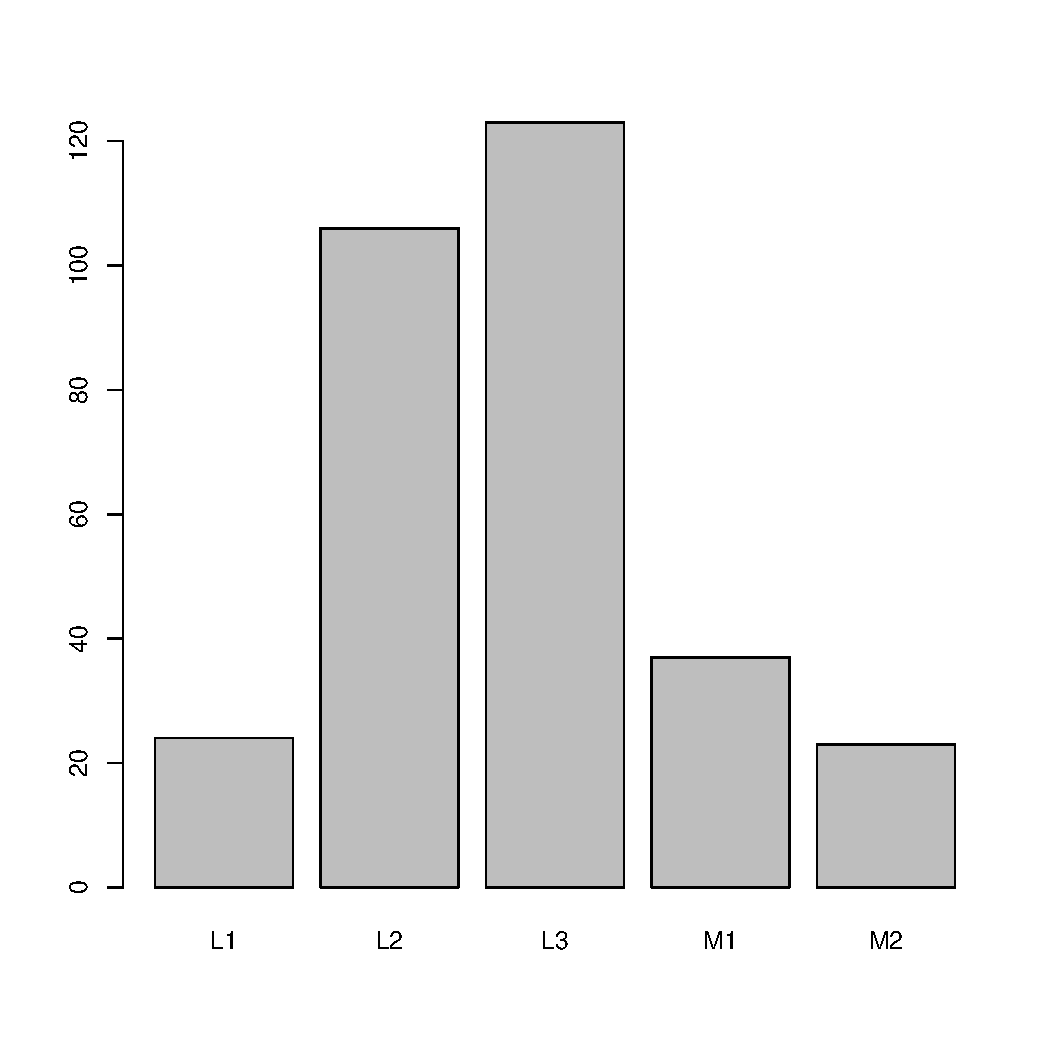
\includegraphics[width=3cm]{graphUniv/V-barplot}
          \end{tabular}
      \\ \hline 

    \end{tabular}
  \end{center}
  
 ee 
